\begin{figure}[H] \centering % Created by tikzDevice version 0.12.4 on 2023-07-18 18:29:49
% !TEX encoding = UTF-8 Unicode
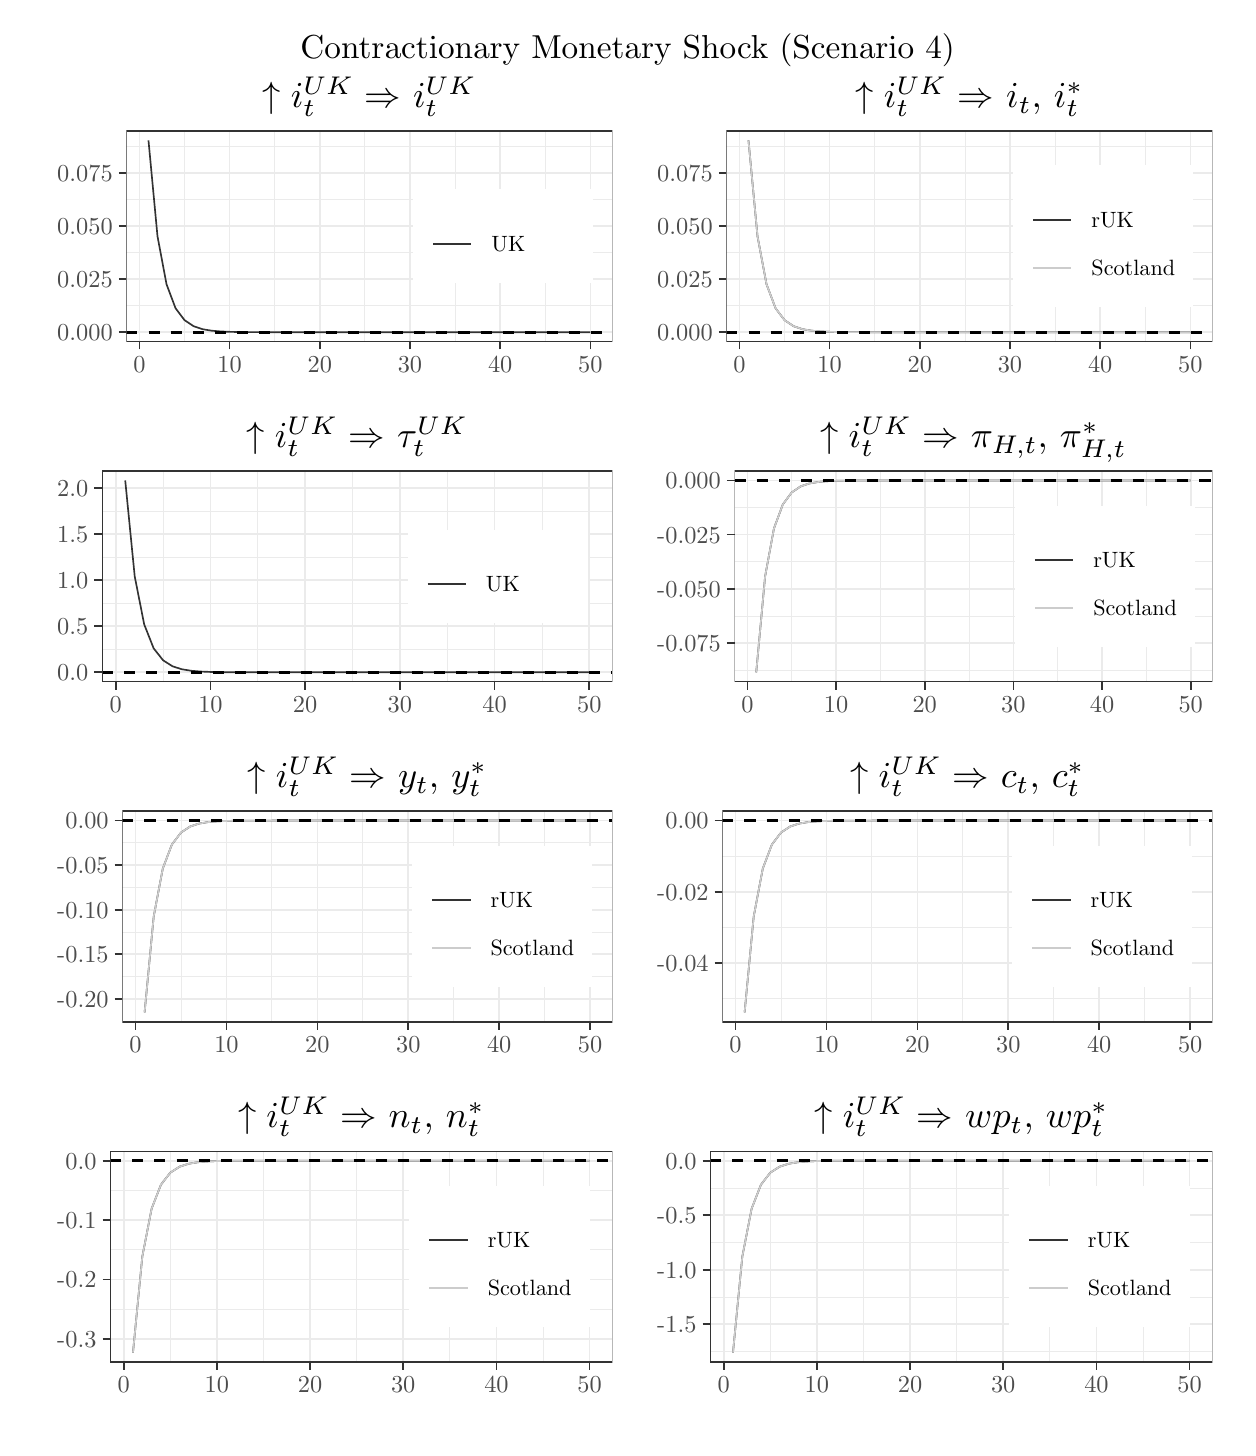
\begin{tikzpicture}[x=1pt,y=1pt]
\definecolor{fillColor}{RGB}{255,255,255}
\path[use as bounding box,fill=fillColor,fill opacity=0.00] (0,0) rectangle (433.62,505.89);
\begin{scope}
\path[clip] (  0.00,368.70) rectangle (216.81,491.60);
\definecolor{drawColor}{RGB}{255,255,255}
\definecolor{fillColor}{RGB}{255,255,255}

\path[draw=drawColor,line width= 0.6pt,line join=round,line cap=round,fill=fillColor] (  0.00,368.70) rectangle (216.81,491.60);
\end{scope}
\begin{scope}
\path[clip] ( 35.67,392.38) rectangle (211.31,468.64);
\definecolor{fillColor}{RGB}{255,255,255}

\path[fill=fillColor] ( 35.67,392.38) rectangle (211.31,468.64);
\definecolor{drawColor}{gray}{0.92}

\path[draw=drawColor,line width= 0.3pt,line join=round] ( 35.67,405.44) --
	(211.31,405.44);

\path[draw=drawColor,line width= 0.3pt,line join=round] ( 35.67,424.63) --
	(211.31,424.63);

\path[draw=drawColor,line width= 0.3pt,line join=round] ( 35.67,443.82) --
	(211.31,443.82);

\path[draw=drawColor,line width= 0.3pt,line join=round] ( 35.67,463.02) --
	(211.31,463.02);

\path[draw=drawColor,line width= 0.3pt,line join=round] ( 56.69,392.38) --
	( 56.69,468.64);

\path[draw=drawColor,line width= 0.3pt,line join=round] ( 89.27,392.38) --
	( 89.27,468.64);

\path[draw=drawColor,line width= 0.3pt,line join=round] (121.86,392.38) --
	(121.86,468.64);

\path[draw=drawColor,line width= 0.3pt,line join=round] (154.45,392.38) --
	(154.45,468.64);

\path[draw=drawColor,line width= 0.3pt,line join=round] (187.03,392.38) --
	(187.03,468.64);

\path[draw=drawColor,line width= 0.6pt,line join=round] ( 35.67,395.85) --
	(211.31,395.85);

\path[draw=drawColor,line width= 0.6pt,line join=round] ( 35.67,415.04) --
	(211.31,415.04);

\path[draw=drawColor,line width= 0.6pt,line join=round] ( 35.67,434.23) --
	(211.31,434.23);

\path[draw=drawColor,line width= 0.6pt,line join=round] ( 35.67,453.42) --
	(211.31,453.42);

\path[draw=drawColor,line width= 0.6pt,line join=round] ( 40.39,392.38) --
	( 40.39,468.64);

\path[draw=drawColor,line width= 0.6pt,line join=round] ( 72.98,392.38) --
	( 72.98,468.64);

\path[draw=drawColor,line width= 0.6pt,line join=round] (105.57,392.38) --
	(105.57,468.64);

\path[draw=drawColor,line width= 0.6pt,line join=round] (138.15,392.38) --
	(138.15,468.64);

\path[draw=drawColor,line width= 0.6pt,line join=round] (170.74,392.38) --
	(170.74,468.64);

\path[draw=drawColor,line width= 0.6pt,line join=round] (203.33,392.38) --
	(203.33,468.64);
\definecolor{drawColor}{gray}{0.20}

\path[draw=drawColor,line width= 0.6pt,line join=round] ( 43.65,465.17) --
	( 46.91,430.51) --
	( 50.17,413.18) --
	( 53.43,404.51) --
	( 56.69,400.18) --
	( 59.95,398.01) --
	( 63.20,396.93) --
	( 66.46,396.39) --
	( 69.72,396.12) --
	( 72.98,395.98) --
	( 76.24,395.91) --
	( 79.50,395.88) --
	( 82.76,395.86) --
	( 86.01,395.85) --
	( 89.27,395.85) --
	( 92.53,395.85) --
	( 95.79,395.85) --
	( 99.05,395.85) --
	(102.31,395.85) --
	(105.57,395.85) --
	(108.83,395.85) --
	(112.08,395.85) --
	(115.34,395.85) --
	(118.60,395.85) --
	(121.86,395.85) --
	(125.12,395.85) --
	(128.38,395.85) --
	(131.64,395.85) --
	(134.89,395.85) --
	(138.15,395.85) --
	(141.41,395.85) --
	(144.67,395.85) --
	(147.93,395.85) --
	(151.19,395.85) --
	(154.45,395.85) --
	(157.71,395.85) --
	(160.96,395.85) --
	(164.22,395.85) --
	(167.48,395.85) --
	(170.74,395.85) --
	(174.00,395.85) --
	(177.26,395.85) --
	(180.52,395.85) --
	(183.77,395.85) --
	(187.03,395.85) --
	(190.29,395.85) --
	(193.55,395.85) --
	(196.81,395.85) --
	(200.07,395.85) --
	(203.33,395.85);
\definecolor{drawColor}{RGB}{0,0,0}

\path[draw=drawColor,line width= 1.1pt,dash pattern=on 4pt off 4pt ,line join=round] ( 35.67,395.85) -- (211.31,395.85);
\definecolor{drawColor}{gray}{0.20}

\path[draw=drawColor,line width= 0.6pt,line join=round,line cap=round] ( 35.67,392.38) rectangle (211.31,468.64);
\end{scope}
\begin{scope}
\path[clip] (  0.00,  0.00) rectangle (433.62,505.89);
\definecolor{drawColor}{gray}{0.30}

\node[text=drawColor,anchor=base east,inner sep=0pt, outer sep=0pt, scale=  0.88] at ( 30.72,392.82) {0.000};

\node[text=drawColor,anchor=base east,inner sep=0pt, outer sep=0pt, scale=  0.88] at ( 30.72,412.01) {0.025};

\node[text=drawColor,anchor=base east,inner sep=0pt, outer sep=0pt, scale=  0.88] at ( 30.72,431.20) {0.050};

\node[text=drawColor,anchor=base east,inner sep=0pt, outer sep=0pt, scale=  0.88] at ( 30.72,450.39) {0.075};
\end{scope}
\begin{scope}
\path[clip] (  0.00,  0.00) rectangle (433.62,505.89);
\definecolor{drawColor}{gray}{0.20}

\path[draw=drawColor,line width= 0.6pt,line join=round] ( 32.92,395.85) --
	( 35.67,395.85);

\path[draw=drawColor,line width= 0.6pt,line join=round] ( 32.92,415.04) --
	( 35.67,415.04);

\path[draw=drawColor,line width= 0.6pt,line join=round] ( 32.92,434.23) --
	( 35.67,434.23);

\path[draw=drawColor,line width= 0.6pt,line join=round] ( 32.92,453.42) --
	( 35.67,453.42);
\end{scope}
\begin{scope}
\path[clip] (  0.00,  0.00) rectangle (433.62,505.89);
\definecolor{drawColor}{gray}{0.20}

\path[draw=drawColor,line width= 0.6pt,line join=round] ( 40.39,389.63) --
	( 40.39,392.38);

\path[draw=drawColor,line width= 0.6pt,line join=round] ( 72.98,389.63) --
	( 72.98,392.38);

\path[draw=drawColor,line width= 0.6pt,line join=round] (105.57,389.63) --
	(105.57,392.38);

\path[draw=drawColor,line width= 0.6pt,line join=round] (138.15,389.63) --
	(138.15,392.38);

\path[draw=drawColor,line width= 0.6pt,line join=round] (170.74,389.63) --
	(170.74,392.38);

\path[draw=drawColor,line width= 0.6pt,line join=round] (203.33,389.63) --
	(203.33,392.38);
\end{scope}
\begin{scope}
\path[clip] (  0.00,  0.00) rectangle (433.62,505.89);
\definecolor{drawColor}{gray}{0.30}

\node[text=drawColor,anchor=base,inner sep=0pt, outer sep=0pt, scale=  0.88] at ( 40.39,381.37) {0};

\node[text=drawColor,anchor=base,inner sep=0pt, outer sep=0pt, scale=  0.88] at ( 72.98,381.37) {10};

\node[text=drawColor,anchor=base,inner sep=0pt, outer sep=0pt, scale=  0.88] at (105.57,381.37) {20};

\node[text=drawColor,anchor=base,inner sep=0pt, outer sep=0pt, scale=  0.88] at (138.15,381.37) {30};

\node[text=drawColor,anchor=base,inner sep=0pt, outer sep=0pt, scale=  0.88] at (170.74,381.37) {40};

\node[text=drawColor,anchor=base,inner sep=0pt, outer sep=0pt, scale=  0.88] at (203.33,381.37) {50};
\end{scope}
\begin{scope}
\path[clip] (  0.00,  0.00) rectangle (433.62,505.89);
\definecolor{fillColor}{RGB}{255,255,255}

\path[fill=fillColor] (139.25,413.59) rectangle (204.34,447.43);
\end{scope}
\begin{scope}
\path[clip] (  0.00,  0.00) rectangle (433.62,505.89);
\definecolor{fillColor}{RGB}{255,255,255}

\path[fill=fillColor] (144.75,419.09) rectangle (162.09,436.43);
\end{scope}
\begin{scope}
\path[clip] (  0.00,  0.00) rectangle (433.62,505.89);
\definecolor{drawColor}{gray}{0.20}

\path[draw=drawColor,line width= 0.6pt,line join=round] (146.48,427.76) -- (160.36,427.76);
\end{scope}
\begin{scope}
\path[clip] (  0.00,  0.00) rectangle (433.62,505.89);
\definecolor{drawColor}{RGB}{0,0,0}

\node[text=drawColor,anchor=base west,inner sep=0pt, outer sep=0pt, scale=  0.80] at (167.59,425.01) {UK};
\end{scope}
\begin{scope}
\path[clip] (  0.00,  0.00) rectangle (433.62,505.89);
\definecolor{drawColor}{RGB}{0,0,0}

\node[text=drawColor,anchor=base,inner sep=0pt, outer sep=0pt, scale=  1.32] at (123.49,477.01) {$\uparrow  i^{UK}_t \Rightarrow $ ${i^{UK}_t}$};
\end{scope}
\begin{scope}
\path[clip] (216.81,368.70) rectangle (433.62,491.60);
\definecolor{drawColor}{RGB}{255,255,255}
\definecolor{fillColor}{RGB}{255,255,255}

\path[draw=drawColor,line width= 0.6pt,line join=round,line cap=round,fill=fillColor] (216.81,368.70) rectangle (433.62,491.60);
\end{scope}
\begin{scope}
\path[clip] (252.48,392.38) rectangle (428.12,468.64);
\definecolor{fillColor}{RGB}{255,255,255}

\path[fill=fillColor] (252.48,392.38) rectangle (428.12,468.64);
\definecolor{drawColor}{gray}{0.92}

\path[draw=drawColor,line width= 0.3pt,line join=round] (252.48,405.44) --
	(428.12,405.44);

\path[draw=drawColor,line width= 0.3pt,line join=round] (252.48,424.63) --
	(428.12,424.63);

\path[draw=drawColor,line width= 0.3pt,line join=round] (252.48,443.82) --
	(428.12,443.82);

\path[draw=drawColor,line width= 0.3pt,line join=round] (252.48,463.02) --
	(428.12,463.02);

\path[draw=drawColor,line width= 0.3pt,line join=round] (273.50,392.38) --
	(273.50,468.64);

\path[draw=drawColor,line width= 0.3pt,line join=round] (306.08,392.38) --
	(306.08,468.64);

\path[draw=drawColor,line width= 0.3pt,line join=round] (338.67,392.38) --
	(338.67,468.64);

\path[draw=drawColor,line width= 0.3pt,line join=round] (371.26,392.38) --
	(371.26,468.64);

\path[draw=drawColor,line width= 0.3pt,line join=round] (403.84,392.38) --
	(403.84,468.64);

\path[draw=drawColor,line width= 0.6pt,line join=round] (252.48,395.85) --
	(428.12,395.85);

\path[draw=drawColor,line width= 0.6pt,line join=round] (252.48,415.04) --
	(428.12,415.04);

\path[draw=drawColor,line width= 0.6pt,line join=round] (252.48,434.23) --
	(428.12,434.23);

\path[draw=drawColor,line width= 0.6pt,line join=round] (252.48,453.42) --
	(428.12,453.42);

\path[draw=drawColor,line width= 0.6pt,line join=round] (257.20,392.38) --
	(257.20,468.64);

\path[draw=drawColor,line width= 0.6pt,line join=round] (289.79,392.38) --
	(289.79,468.64);

\path[draw=drawColor,line width= 0.6pt,line join=round] (322.38,392.38) --
	(322.38,468.64);

\path[draw=drawColor,line width= 0.6pt,line join=round] (354.96,392.38) --
	(354.96,468.64);

\path[draw=drawColor,line width= 0.6pt,line join=round] (387.55,392.38) --
	(387.55,468.64);

\path[draw=drawColor,line width= 0.6pt,line join=round] (420.14,392.38) --
	(420.14,468.64);
\definecolor{drawColor}{gray}{0.20}

\path[draw=drawColor,line width= 0.6pt,line join=round] (260.46,465.17) --
	(263.72,430.51) --
	(266.98,413.18) --
	(270.24,404.51) --
	(273.50,400.18) --
	(276.76,398.01) --
	(280.01,396.93) --
	(283.27,396.39) --
	(286.53,396.12) --
	(289.79,395.98) --
	(293.05,395.91) --
	(296.31,395.88) --
	(299.57,395.86) --
	(302.82,395.85) --
	(306.08,395.85) --
	(309.34,395.85) --
	(312.60,395.85) --
	(315.86,395.85) --
	(319.12,395.85) --
	(322.38,395.85) --
	(325.64,395.85) --
	(328.89,395.85) --
	(332.15,395.85) --
	(335.41,395.85) --
	(338.67,395.85) --
	(341.93,395.85) --
	(345.19,395.85) --
	(348.45,395.85) --
	(351.70,395.85) --
	(354.96,395.85) --
	(358.22,395.85) --
	(361.48,395.85) --
	(364.74,395.85) --
	(368.00,395.85) --
	(371.26,395.85) --
	(374.52,395.85) --
	(377.77,395.85) --
	(381.03,395.85) --
	(384.29,395.85) --
	(387.55,395.85) --
	(390.81,395.85) --
	(394.07,395.85) --
	(397.33,395.85) --
	(400.58,395.85) --
	(403.84,395.85) --
	(407.10,395.85) --
	(410.36,395.85) --
	(413.62,395.85) --
	(416.88,395.85) --
	(420.14,395.85);
\definecolor{drawColor}{gray}{0.80}

\path[draw=drawColor,line width= 0.6pt,line join=round] (260.46,465.17) --
	(263.72,430.51) --
	(266.98,413.18) --
	(270.24,404.51) --
	(273.50,400.18) --
	(276.76,398.01) --
	(280.01,396.93) --
	(283.27,396.39) --
	(286.53,396.12) --
	(289.79,395.98) --
	(293.05,395.91) --
	(296.31,395.88) --
	(299.57,395.86) --
	(302.82,395.85) --
	(306.08,395.85) --
	(309.34,395.85) --
	(312.60,395.85) --
	(315.86,395.85) --
	(319.12,395.85) --
	(322.38,395.85) --
	(325.64,395.85) --
	(328.89,395.85) --
	(332.15,395.85) --
	(335.41,395.85) --
	(338.67,395.85) --
	(341.93,395.85) --
	(345.19,395.85) --
	(348.45,395.85) --
	(351.70,395.85) --
	(354.96,395.85) --
	(358.22,395.85) --
	(361.48,395.85) --
	(364.74,395.85) --
	(368.00,395.85) --
	(371.26,395.85) --
	(374.52,395.85) --
	(377.77,395.85) --
	(381.03,395.85) --
	(384.29,395.85) --
	(387.55,395.85) --
	(390.81,395.85) --
	(394.07,395.85) --
	(397.33,395.85) --
	(400.58,395.85) --
	(403.84,395.85) --
	(407.10,395.85) --
	(410.36,395.85) --
	(413.62,395.85) --
	(416.88,395.85) --
	(420.14,395.85);
\definecolor{drawColor}{RGB}{0,0,0}

\path[draw=drawColor,line width= 1.1pt,dash pattern=on 4pt off 4pt ,line join=round] (252.48,395.85) -- (428.12,395.85);
\definecolor{drawColor}{gray}{0.20}

\path[draw=drawColor,line width= 0.6pt,line join=round,line cap=round] (252.48,392.38) rectangle (428.12,468.64);
\end{scope}
\begin{scope}
\path[clip] (  0.00,  0.00) rectangle (433.62,505.89);
\definecolor{drawColor}{gray}{0.30}

\node[text=drawColor,anchor=base east,inner sep=0pt, outer sep=0pt, scale=  0.88] at (247.53,392.82) {0.000};

\node[text=drawColor,anchor=base east,inner sep=0pt, outer sep=0pt, scale=  0.88] at (247.53,412.01) {0.025};

\node[text=drawColor,anchor=base east,inner sep=0pt, outer sep=0pt, scale=  0.88] at (247.53,431.20) {0.050};

\node[text=drawColor,anchor=base east,inner sep=0pt, outer sep=0pt, scale=  0.88] at (247.53,450.39) {0.075};
\end{scope}
\begin{scope}
\path[clip] (  0.00,  0.00) rectangle (433.62,505.89);
\definecolor{drawColor}{gray}{0.20}

\path[draw=drawColor,line width= 0.6pt,line join=round] (249.73,395.85) --
	(252.48,395.85);

\path[draw=drawColor,line width= 0.6pt,line join=round] (249.73,415.04) --
	(252.48,415.04);

\path[draw=drawColor,line width= 0.6pt,line join=round] (249.73,434.23) --
	(252.48,434.23);

\path[draw=drawColor,line width= 0.6pt,line join=round] (249.73,453.42) --
	(252.48,453.42);
\end{scope}
\begin{scope}
\path[clip] (  0.00,  0.00) rectangle (433.62,505.89);
\definecolor{drawColor}{gray}{0.20}

\path[draw=drawColor,line width= 0.6pt,line join=round] (257.20,389.63) --
	(257.20,392.38);

\path[draw=drawColor,line width= 0.6pt,line join=round] (289.79,389.63) --
	(289.79,392.38);

\path[draw=drawColor,line width= 0.6pt,line join=round] (322.38,389.63) --
	(322.38,392.38);

\path[draw=drawColor,line width= 0.6pt,line join=round] (354.96,389.63) --
	(354.96,392.38);

\path[draw=drawColor,line width= 0.6pt,line join=round] (387.55,389.63) --
	(387.55,392.38);

\path[draw=drawColor,line width= 0.6pt,line join=round] (420.14,389.63) --
	(420.14,392.38);
\end{scope}
\begin{scope}
\path[clip] (  0.00,  0.00) rectangle (433.62,505.89);
\definecolor{drawColor}{gray}{0.30}

\node[text=drawColor,anchor=base,inner sep=0pt, outer sep=0pt, scale=  0.88] at (257.20,381.37) {0};

\node[text=drawColor,anchor=base,inner sep=0pt, outer sep=0pt, scale=  0.88] at (289.79,381.37) {10};

\node[text=drawColor,anchor=base,inner sep=0pt, outer sep=0pt, scale=  0.88] at (322.38,381.37) {20};

\node[text=drawColor,anchor=base,inner sep=0pt, outer sep=0pt, scale=  0.88] at (354.96,381.37) {30};

\node[text=drawColor,anchor=base,inner sep=0pt, outer sep=0pt, scale=  0.88] at (387.55,381.37) {40};

\node[text=drawColor,anchor=base,inner sep=0pt, outer sep=0pt, scale=  0.88] at (420.14,381.37) {50};
\end{scope}
\begin{scope}
\path[clip] (  0.00,  0.00) rectangle (433.62,505.89);
\definecolor{fillColor}{RGB}{255,255,255}

\path[fill=fillColor] (356.06,404.92) rectangle (421.15,456.11);
\end{scope}
\begin{scope}
\path[clip] (  0.00,  0.00) rectangle (433.62,505.89);
\definecolor{fillColor}{RGB}{255,255,255}

\path[fill=fillColor] (361.56,427.76) rectangle (378.90,445.11);
\end{scope}
\begin{scope}
\path[clip] (  0.00,  0.00) rectangle (433.62,505.89);
\definecolor{drawColor}{gray}{0.20}

\path[draw=drawColor,line width= 0.6pt,line join=round] (363.29,436.43) -- (377.17,436.43);
\end{scope}
\begin{scope}
\path[clip] (  0.00,  0.00) rectangle (433.62,505.89);
\definecolor{fillColor}{RGB}{255,255,255}

\path[fill=fillColor] (361.56,410.42) rectangle (378.90,427.76);
\end{scope}
\begin{scope}
\path[clip] (  0.00,  0.00) rectangle (433.62,505.89);
\definecolor{drawColor}{gray}{0.80}

\path[draw=drawColor,line width= 0.6pt,line join=round] (363.29,419.09) -- (377.17,419.09);
\end{scope}
\begin{scope}
\path[clip] (  0.00,  0.00) rectangle (433.62,505.89);
\definecolor{drawColor}{RGB}{0,0,0}

\node[text=drawColor,anchor=base west,inner sep=0pt, outer sep=0pt, scale=  0.80] at (384.40,433.68) {rUK};
\end{scope}
\begin{scope}
\path[clip] (  0.00,  0.00) rectangle (433.62,505.89);
\definecolor{drawColor}{RGB}{0,0,0}

\node[text=drawColor,anchor=base west,inner sep=0pt, outer sep=0pt, scale=  0.80] at (384.40,416.33) {Scotland};
\end{scope}
\begin{scope}
\path[clip] (  0.00,  0.00) rectangle (433.62,505.89);
\definecolor{drawColor}{RGB}{0,0,0}

\node[text=drawColor,anchor=base,inner sep=0pt, outer sep=0pt, scale=  1.32] at (340.30,477.01) {$\uparrow  i^{UK}_t \Rightarrow $ ${i_t}$, ${i^*_t}$};
\end{scope}
\begin{scope}
\path[clip] (  0.00,245.80) rectangle (216.81,368.70);
\definecolor{drawColor}{RGB}{255,255,255}
\definecolor{fillColor}{RGB}{255,255,255}

\path[draw=drawColor,line width= 0.6pt,line join=round,line cap=round,fill=fillColor] (  0.00,245.80) rectangle (216.81,368.70);
\end{scope}
\begin{scope}
\path[clip] ( 26.87,269.48) rectangle (211.31,345.74);
\definecolor{fillColor}{RGB}{255,255,255}

\path[fill=fillColor] ( 26.87,269.48) rectangle (211.31,345.74);
\definecolor{drawColor}{gray}{0.92}

\path[draw=drawColor,line width= 0.3pt,line join=round] ( 26.87,281.27) --
	(211.31,281.27);

\path[draw=drawColor,line width= 0.3pt,line join=round] ( 26.87,297.91) --
	(211.31,297.91);

\path[draw=drawColor,line width= 0.3pt,line join=round] ( 26.87,314.55) --
	(211.31,314.55);

\path[draw=drawColor,line width= 0.3pt,line join=round] ( 26.87,331.19) --
	(211.31,331.19);

\path[draw=drawColor,line width= 0.3pt,line join=round] ( 48.94,269.48) --
	( 48.94,345.74);

\path[draw=drawColor,line width= 0.3pt,line join=round] ( 83.16,269.48) --
	( 83.16,345.74);

\path[draw=drawColor,line width= 0.3pt,line join=round] (117.38,269.48) --
	(117.38,345.74);

\path[draw=drawColor,line width= 0.3pt,line join=round] (151.60,269.48) --
	(151.60,345.74);

\path[draw=drawColor,line width= 0.3pt,line join=round] (185.82,269.48) --
	(185.82,345.74);

\path[draw=drawColor,line width= 0.6pt,line join=round] ( 26.87,272.95) --
	(211.31,272.95);

\path[draw=drawColor,line width= 0.6pt,line join=round] ( 26.87,289.59) --
	(211.31,289.59);

\path[draw=drawColor,line width= 0.6pt,line join=round] ( 26.87,306.23) --
	(211.31,306.23);

\path[draw=drawColor,line width= 0.6pt,line join=round] ( 26.87,322.87) --
	(211.31,322.87);

\path[draw=drawColor,line width= 0.6pt,line join=round] ( 26.87,339.51) --
	(211.31,339.51);

\path[draw=drawColor,line width= 0.6pt,line join=round] ( 31.83,269.48) --
	( 31.83,345.74);

\path[draw=drawColor,line width= 0.6pt,line join=round] ( 66.05,269.48) --
	( 66.05,345.74);

\path[draw=drawColor,line width= 0.6pt,line join=round] (100.27,269.48) --
	(100.27,345.74);

\path[draw=drawColor,line width= 0.6pt,line join=round] (134.49,269.48) --
	(134.49,345.74);

\path[draw=drawColor,line width= 0.6pt,line join=round] (168.71,269.48) --
	(168.71,345.74);

\path[draw=drawColor,line width= 0.6pt,line join=round] (202.93,269.48) --
	(202.93,345.74);
\definecolor{drawColor}{gray}{0.20}

\path[draw=drawColor,line width= 0.6pt,line join=round] ( 35.25,342.27) --
	( 38.68,307.61) --
	( 42.10,290.28) --
	( 45.52,281.61) --
	( 48.94,277.28) --
	( 52.36,275.11) --
	( 55.79,274.03) --
	( 59.21,273.49) --
	( 62.63,273.22) --
	( 66.05,273.08) --
	( 69.47,273.01) --
	( 72.90,272.98) --
	( 76.32,272.96) --
	( 79.74,272.95) --
	( 83.16,272.95) --
	( 86.58,272.95) --
	( 90.00,272.95) --
	( 93.43,272.95) --
	( 96.85,272.95) --
	(100.27,272.95) --
	(103.69,272.95) --
	(107.11,272.95) --
	(110.54,272.95) --
	(113.96,272.95) --
	(117.38,272.95) --
	(120.80,272.95) --
	(124.22,272.95) --
	(127.65,272.95) --
	(131.07,272.95) --
	(134.49,272.95) --
	(137.91,272.95) --
	(141.33,272.95) --
	(144.75,272.95) --
	(148.18,272.95) --
	(151.60,272.95) --
	(155.02,272.95) --
	(158.44,272.95) --
	(161.86,272.95) --
	(165.29,272.95) --
	(168.71,272.95) --
	(172.13,272.95) --
	(175.55,272.95) --
	(178.97,272.95) --
	(182.40,272.95) --
	(185.82,272.95) --
	(189.24,272.95) --
	(192.66,272.95) --
	(196.08,272.95) --
	(199.50,272.95) --
	(202.93,272.95);
\definecolor{drawColor}{RGB}{0,0,0}

\path[draw=drawColor,line width= 1.1pt,dash pattern=on 4pt off 4pt ,line join=round] ( 26.87,272.95) -- (211.31,272.95);
\definecolor{drawColor}{gray}{0.20}

\path[draw=drawColor,line width= 0.6pt,line join=round,line cap=round] ( 26.87,269.48) rectangle (211.31,345.74);
\end{scope}
\begin{scope}
\path[clip] (  0.00,  0.00) rectangle (433.62,505.89);
\definecolor{drawColor}{gray}{0.30}

\node[text=drawColor,anchor=base east,inner sep=0pt, outer sep=0pt, scale=  0.88] at ( 21.92,269.91) {0.0};

\node[text=drawColor,anchor=base east,inner sep=0pt, outer sep=0pt, scale=  0.88] at ( 21.92,286.56) {0.5};

\node[text=drawColor,anchor=base east,inner sep=0pt, outer sep=0pt, scale=  0.88] at ( 21.92,303.20) {1.0};

\node[text=drawColor,anchor=base east,inner sep=0pt, outer sep=0pt, scale=  0.88] at ( 21.92,319.84) {1.5};

\node[text=drawColor,anchor=base east,inner sep=0pt, outer sep=0pt, scale=  0.88] at ( 21.92,336.48) {2.0};
\end{scope}
\begin{scope}
\path[clip] (  0.00,  0.00) rectangle (433.62,505.89);
\definecolor{drawColor}{gray}{0.20}

\path[draw=drawColor,line width= 0.6pt,line join=round] ( 24.12,272.95) --
	( 26.87,272.95);

\path[draw=drawColor,line width= 0.6pt,line join=round] ( 24.12,289.59) --
	( 26.87,289.59);

\path[draw=drawColor,line width= 0.6pt,line join=round] ( 24.12,306.23) --
	( 26.87,306.23);

\path[draw=drawColor,line width= 0.6pt,line join=round] ( 24.12,322.87) --
	( 26.87,322.87);

\path[draw=drawColor,line width= 0.6pt,line join=round] ( 24.12,339.51) --
	( 26.87,339.51);
\end{scope}
\begin{scope}
\path[clip] (  0.00,  0.00) rectangle (433.62,505.89);
\definecolor{drawColor}{gray}{0.20}

\path[draw=drawColor,line width= 0.6pt,line join=round] ( 31.83,266.73) --
	( 31.83,269.48);

\path[draw=drawColor,line width= 0.6pt,line join=round] ( 66.05,266.73) --
	( 66.05,269.48);

\path[draw=drawColor,line width= 0.6pt,line join=round] (100.27,266.73) --
	(100.27,269.48);

\path[draw=drawColor,line width= 0.6pt,line join=round] (134.49,266.73) --
	(134.49,269.48);

\path[draw=drawColor,line width= 0.6pt,line join=round] (168.71,266.73) --
	(168.71,269.48);

\path[draw=drawColor,line width= 0.6pt,line join=round] (202.93,266.73) --
	(202.93,269.48);
\end{scope}
\begin{scope}
\path[clip] (  0.00,  0.00) rectangle (433.62,505.89);
\definecolor{drawColor}{gray}{0.30}

\node[text=drawColor,anchor=base,inner sep=0pt, outer sep=0pt, scale=  0.88] at ( 31.83,258.47) {0};

\node[text=drawColor,anchor=base,inner sep=0pt, outer sep=0pt, scale=  0.88] at ( 66.05,258.47) {10};

\node[text=drawColor,anchor=base,inner sep=0pt, outer sep=0pt, scale=  0.88] at (100.27,258.47) {20};

\node[text=drawColor,anchor=base,inner sep=0pt, outer sep=0pt, scale=  0.88] at (134.49,258.47) {30};

\node[text=drawColor,anchor=base,inner sep=0pt, outer sep=0pt, scale=  0.88] at (168.71,258.47) {40};

\node[text=drawColor,anchor=base,inner sep=0pt, outer sep=0pt, scale=  0.88] at (202.93,258.47) {50};
\end{scope}
\begin{scope}
\path[clip] (  0.00,  0.00) rectangle (433.62,505.89);
\definecolor{fillColor}{RGB}{255,255,255}

\path[fill=fillColor] (137.27,290.69) rectangle (202.36,324.53);
\end{scope}
\begin{scope}
\path[clip] (  0.00,  0.00) rectangle (433.62,505.89);
\definecolor{fillColor}{RGB}{255,255,255}

\path[fill=fillColor] (142.77,296.19) rectangle (160.11,313.53);
\end{scope}
\begin{scope}
\path[clip] (  0.00,  0.00) rectangle (433.62,505.89);
\definecolor{drawColor}{gray}{0.20}

\path[draw=drawColor,line width= 0.6pt,line join=round] (144.50,304.86) -- (158.38,304.86);
\end{scope}
\begin{scope}
\path[clip] (  0.00,  0.00) rectangle (433.62,505.89);
\definecolor{drawColor}{RGB}{0,0,0}

\node[text=drawColor,anchor=base west,inner sep=0pt, outer sep=0pt, scale=  0.80] at (165.61,302.10) {UK};
\end{scope}
\begin{scope}
\path[clip] (  0.00,  0.00) rectangle (433.62,505.89);
\definecolor{drawColor}{RGB}{0,0,0}

\node[text=drawColor,anchor=base,inner sep=0pt, outer sep=0pt, scale=  1.32] at (119.09,354.11) {$\uparrow  i^{UK}_t \Rightarrow $ ${\tau^{UK}_t}$};
\end{scope}
\begin{scope}
\path[clip] (216.81,245.80) rectangle (433.62,368.70);
\definecolor{drawColor}{RGB}{255,255,255}
\definecolor{fillColor}{RGB}{255,255,255}

\path[draw=drawColor,line width= 0.6pt,line join=round,line cap=round,fill=fillColor] (216.81,245.80) rectangle (433.62,368.70);
\end{scope}
\begin{scope}
\path[clip] (255.41,269.48) rectangle (428.12,345.74);
\definecolor{fillColor}{RGB}{255,255,255}

\path[fill=fillColor] (255.41,269.48) rectangle (428.12,345.74);
\definecolor{drawColor}{gray}{0.92}

\path[draw=drawColor,line width= 0.3pt,line join=round] (255.41,273.74) --
	(428.12,273.74);

\path[draw=drawColor,line width= 0.3pt,line join=round] (255.41,293.32) --
	(428.12,293.32);

\path[draw=drawColor,line width= 0.3pt,line join=round] (255.41,312.90) --
	(428.12,312.90);

\path[draw=drawColor,line width= 0.3pt,line join=round] (255.41,332.48) --
	(428.12,332.48);

\path[draw=drawColor,line width= 0.3pt,line join=round] (276.08,269.48) --
	(276.08,345.74);

\path[draw=drawColor,line width= 0.3pt,line join=round] (308.12,269.48) --
	(308.12,345.74);

\path[draw=drawColor,line width= 0.3pt,line join=round] (340.16,269.48) --
	(340.16,345.74);

\path[draw=drawColor,line width= 0.3pt,line join=round] (372.21,269.48) --
	(372.21,345.74);

\path[draw=drawColor,line width= 0.3pt,line join=round] (404.25,269.48) --
	(404.25,345.74);

\path[draw=drawColor,line width= 0.6pt,line join=round] (255.41,283.53) --
	(428.12,283.53);

\path[draw=drawColor,line width= 0.6pt,line join=round] (255.41,303.11) --
	(428.12,303.11);

\path[draw=drawColor,line width= 0.6pt,line join=round] (255.41,322.69) --
	(428.12,322.69);

\path[draw=drawColor,line width= 0.6pt,line join=round] (255.41,342.27) --
	(428.12,342.27);

\path[draw=drawColor,line width= 0.6pt,line join=round] (260.06,269.48) --
	(260.06,345.74);

\path[draw=drawColor,line width= 0.6pt,line join=round] (292.10,269.48) --
	(292.10,345.74);

\path[draw=drawColor,line width= 0.6pt,line join=round] (324.14,269.48) --
	(324.14,345.74);

\path[draw=drawColor,line width= 0.6pt,line join=round] (356.18,269.48) --
	(356.18,345.74);

\path[draw=drawColor,line width= 0.6pt,line join=round] (388.23,269.48) --
	(388.23,345.74);

\path[draw=drawColor,line width= 0.6pt,line join=round] (420.27,269.48) --
	(420.27,345.74);
\definecolor{drawColor}{gray}{0.20}

\path[draw=drawColor,line width= 0.6pt,line join=round] (263.26,272.95) --
	(266.47,307.61) --
	(269.67,324.94) --
	(272.87,333.61) --
	(276.08,337.94) --
	(279.28,340.11) --
	(282.49,341.19) --
	(285.69,341.73) --
	(288.90,342.00) --
	(292.10,342.14) --
	(295.30,342.21) --
	(298.51,342.24) --
	(301.71,342.26) --
	(304.92,342.27) --
	(308.12,342.27) --
	(311.33,342.27) --
	(314.53,342.27) --
	(317.73,342.27) --
	(320.94,342.27) --
	(324.14,342.27) --
	(327.35,342.27) --
	(330.55,342.27) --
	(333.76,342.27) --
	(336.96,342.27) --
	(340.16,342.27) --
	(343.37,342.27) --
	(346.57,342.27) --
	(349.78,342.27) --
	(352.98,342.27) --
	(356.18,342.27) --
	(359.39,342.27) --
	(362.59,342.27) --
	(365.80,342.27) --
	(369.00,342.27) --
	(372.21,342.27) --
	(375.41,342.27) --
	(378.61,342.27) --
	(381.82,342.27) --
	(385.02,342.27) --
	(388.23,342.27) --
	(391.43,342.27) --
	(394.64,342.27) --
	(397.84,342.27) --
	(401.04,342.27) --
	(404.25,342.27) --
	(407.45,342.27) --
	(410.66,342.27) --
	(413.86,342.27) --
	(417.07,342.27) --
	(420.27,342.27);
\definecolor{drawColor}{gray}{0.80}

\path[draw=drawColor,line width= 0.6pt,line join=round] (263.26,272.95) --
	(266.47,307.61) --
	(269.67,324.94) --
	(272.87,333.61) --
	(276.08,337.94) --
	(279.28,340.11) --
	(282.49,341.19) --
	(285.69,341.73) --
	(288.90,342.00) --
	(292.10,342.14) --
	(295.30,342.21) --
	(298.51,342.24) --
	(301.71,342.26) --
	(304.92,342.27) --
	(308.12,342.27) --
	(311.33,342.27) --
	(314.53,342.27) --
	(317.73,342.27) --
	(320.94,342.27) --
	(324.14,342.27) --
	(327.35,342.27) --
	(330.55,342.27) --
	(333.76,342.27) --
	(336.96,342.27) --
	(340.16,342.27) --
	(343.37,342.27) --
	(346.57,342.27) --
	(349.78,342.27) --
	(352.98,342.27) --
	(356.18,342.27) --
	(359.39,342.27) --
	(362.59,342.27) --
	(365.80,342.27) --
	(369.00,342.27) --
	(372.21,342.27) --
	(375.41,342.27) --
	(378.61,342.27) --
	(381.82,342.27) --
	(385.02,342.27) --
	(388.23,342.27) --
	(391.43,342.27) --
	(394.64,342.27) --
	(397.84,342.27) --
	(401.04,342.27) --
	(404.25,342.27) --
	(407.45,342.27) --
	(410.66,342.27) --
	(413.86,342.27) --
	(417.07,342.27) --
	(420.27,342.27);
\definecolor{drawColor}{RGB}{0,0,0}

\path[draw=drawColor,line width= 1.1pt,dash pattern=on 4pt off 4pt ,line join=round] (255.41,342.27) -- (428.12,342.27);
\definecolor{drawColor}{gray}{0.20}

\path[draw=drawColor,line width= 0.6pt,line join=round,line cap=round] (255.41,269.48) rectangle (428.12,345.74);
\end{scope}
\begin{scope}
\path[clip] (  0.00,  0.00) rectangle (433.62,505.89);
\definecolor{drawColor}{gray}{0.30}

\node[text=drawColor,anchor=base east,inner sep=0pt, outer sep=0pt, scale=  0.88] at (250.46,280.50) {-0.075};

\node[text=drawColor,anchor=base east,inner sep=0pt, outer sep=0pt, scale=  0.88] at (250.46,300.08) {-0.050};

\node[text=drawColor,anchor=base east,inner sep=0pt, outer sep=0pt, scale=  0.88] at (250.46,319.66) {-0.025};

\node[text=drawColor,anchor=base east,inner sep=0pt, outer sep=0pt, scale=  0.88] at (250.46,339.24) {0.000};
\end{scope}
\begin{scope}
\path[clip] (  0.00,  0.00) rectangle (433.62,505.89);
\definecolor{drawColor}{gray}{0.20}

\path[draw=drawColor,line width= 0.6pt,line join=round] (252.66,283.53) --
	(255.41,283.53);

\path[draw=drawColor,line width= 0.6pt,line join=round] (252.66,303.11) --
	(255.41,303.11);

\path[draw=drawColor,line width= 0.6pt,line join=round] (252.66,322.69) --
	(255.41,322.69);

\path[draw=drawColor,line width= 0.6pt,line join=round] (252.66,342.27) --
	(255.41,342.27);
\end{scope}
\begin{scope}
\path[clip] (  0.00,  0.00) rectangle (433.62,505.89);
\definecolor{drawColor}{gray}{0.20}

\path[draw=drawColor,line width= 0.6pt,line join=round] (260.06,266.73) --
	(260.06,269.48);

\path[draw=drawColor,line width= 0.6pt,line join=round] (292.10,266.73) --
	(292.10,269.48);

\path[draw=drawColor,line width= 0.6pt,line join=round] (324.14,266.73) --
	(324.14,269.48);

\path[draw=drawColor,line width= 0.6pt,line join=round] (356.18,266.73) --
	(356.18,269.48);

\path[draw=drawColor,line width= 0.6pt,line join=round] (388.23,266.73) --
	(388.23,269.48);

\path[draw=drawColor,line width= 0.6pt,line join=round] (420.27,266.73) --
	(420.27,269.48);
\end{scope}
\begin{scope}
\path[clip] (  0.00,  0.00) rectangle (433.62,505.89);
\definecolor{drawColor}{gray}{0.30}

\node[text=drawColor,anchor=base,inner sep=0pt, outer sep=0pt, scale=  0.88] at (260.06,258.47) {0};

\node[text=drawColor,anchor=base,inner sep=0pt, outer sep=0pt, scale=  0.88] at (292.10,258.47) {10};

\node[text=drawColor,anchor=base,inner sep=0pt, outer sep=0pt, scale=  0.88] at (324.14,258.47) {20};

\node[text=drawColor,anchor=base,inner sep=0pt, outer sep=0pt, scale=  0.88] at (356.18,258.47) {30};

\node[text=drawColor,anchor=base,inner sep=0pt, outer sep=0pt, scale=  0.88] at (388.23,258.47) {40};

\node[text=drawColor,anchor=base,inner sep=0pt, outer sep=0pt, scale=  0.88] at (420.27,258.47) {50};
\end{scope}
\begin{scope}
\path[clip] (  0.00,  0.00) rectangle (433.62,505.89);
\definecolor{fillColor}{RGB}{255,255,255}

\path[fill=fillColor] (356.72,282.01) rectangle (421.81,333.20);
\end{scope}
\begin{scope}
\path[clip] (  0.00,  0.00) rectangle (433.62,505.89);
\definecolor{fillColor}{RGB}{255,255,255}

\path[fill=fillColor] (362.22,304.86) rectangle (379.56,322.20);
\end{scope}
\begin{scope}
\path[clip] (  0.00,  0.00) rectangle (433.62,505.89);
\definecolor{drawColor}{gray}{0.20}

\path[draw=drawColor,line width= 0.6pt,line join=round] (363.95,313.53) -- (377.83,313.53);
\end{scope}
\begin{scope}
\path[clip] (  0.00,  0.00) rectangle (433.62,505.89);
\definecolor{fillColor}{RGB}{255,255,255}

\path[fill=fillColor] (362.22,287.51) rectangle (379.56,304.86);
\end{scope}
\begin{scope}
\path[clip] (  0.00,  0.00) rectangle (433.62,505.89);
\definecolor{drawColor}{gray}{0.80}

\path[draw=drawColor,line width= 0.6pt,line join=round] (363.95,296.19) -- (377.83,296.19);
\end{scope}
\begin{scope}
\path[clip] (  0.00,  0.00) rectangle (433.62,505.89);
\definecolor{drawColor}{RGB}{0,0,0}

\node[text=drawColor,anchor=base west,inner sep=0pt, outer sep=0pt, scale=  0.80] at (385.06,310.78) {rUK};
\end{scope}
\begin{scope}
\path[clip] (  0.00,  0.00) rectangle (433.62,505.89);
\definecolor{drawColor}{RGB}{0,0,0}

\node[text=drawColor,anchor=base west,inner sep=0pt, outer sep=0pt, scale=  0.80] at (385.06,293.43) {Scotland};
\end{scope}
\begin{scope}
\path[clip] (  0.00,  0.00) rectangle (433.62,505.89);
\definecolor{drawColor}{RGB}{0,0,0}

\node[text=drawColor,anchor=base,inner sep=0pt, outer sep=0pt, scale=  1.32] at (341.77,354.11) {$\uparrow  i^{UK}_t \Rightarrow $ ${\pi_{H,t}}$, ${\pi^*_{H,t}}$};
\end{scope}
\begin{scope}
\path[clip] (  0.00,122.90) rectangle (216.81,245.80);
\definecolor{drawColor}{RGB}{255,255,255}
\definecolor{fillColor}{RGB}{255,255,255}

\path[draw=drawColor,line width= 0.6pt,line join=round,line cap=round,fill=fillColor] (  0.00,122.90) rectangle (216.81,245.80);
\end{scope}
\begin{scope}
\path[clip] ( 34.20,146.58) rectangle (211.31,222.84);
\definecolor{fillColor}{RGB}{255,255,255}

\path[fill=fillColor] ( 34.20,146.58) rectangle (211.31,222.84);
\definecolor{drawColor}{gray}{0.92}

\path[draw=drawColor,line width= 0.3pt,line join=round] ( 34.20,146.92) --
	(211.31,146.92);

\path[draw=drawColor,line width= 0.3pt,line join=round] ( 34.20,163.02) --
	(211.31,163.02);

\path[draw=drawColor,line width= 0.3pt,line join=round] ( 34.20,179.12) --
	(211.31,179.12);

\path[draw=drawColor,line width= 0.3pt,line join=round] ( 34.20,195.22) --
	(211.31,195.22);

\path[draw=drawColor,line width= 0.3pt,line join=round] ( 34.20,211.32) --
	(211.31,211.32);

\path[draw=drawColor,line width= 0.3pt,line join=round] ( 55.40,146.58) --
	( 55.40,222.84);

\path[draw=drawColor,line width= 0.3pt,line join=round] ( 88.25,146.58) --
	( 88.25,222.84);

\path[draw=drawColor,line width= 0.3pt,line join=round] (121.11,146.58) --
	(121.11,222.84);

\path[draw=drawColor,line width= 0.3pt,line join=round] (153.97,146.58) --
	(153.97,222.84);

\path[draw=drawColor,line width= 0.3pt,line join=round] (186.83,146.58) --
	(186.83,222.84);

\path[draw=drawColor,line width= 0.6pt,line join=round] ( 34.20,154.97) --
	(211.31,154.97);

\path[draw=drawColor,line width= 0.6pt,line join=round] ( 34.20,171.07) --
	(211.31,171.07);

\path[draw=drawColor,line width= 0.6pt,line join=round] ( 34.20,187.17) --
	(211.31,187.17);

\path[draw=drawColor,line width= 0.6pt,line join=round] ( 34.20,203.27) --
	(211.31,203.27);

\path[draw=drawColor,line width= 0.6pt,line join=round] ( 34.20,219.37) --
	(211.31,219.37);

\path[draw=drawColor,line width= 0.6pt,line join=round] ( 38.97,146.58) --
	( 38.97,222.84);

\path[draw=drawColor,line width= 0.6pt,line join=round] ( 71.83,146.58) --
	( 71.83,222.84);

\path[draw=drawColor,line width= 0.6pt,line join=round] (104.68,146.58) --
	(104.68,222.84);

\path[draw=drawColor,line width= 0.6pt,line join=round] (137.54,146.58) --
	(137.54,222.84);

\path[draw=drawColor,line width= 0.6pt,line join=round] (170.40,146.58) --
	(170.40,222.84);

\path[draw=drawColor,line width= 0.6pt,line join=round] (203.26,146.58) --
	(203.26,222.84);
\definecolor{drawColor}{gray}{0.20}

\path[draw=drawColor,line width= 0.6pt,line join=round] ( 42.25,150.04) --
	( 45.54,184.71) --
	( 48.82,202.04) --
	( 52.11,210.71) --
	( 55.40,215.04) --
	( 58.68,217.21) --
	( 61.97,218.29) --
	( 65.25,218.83) --
	( 68.54,219.10) --
	( 71.83,219.24) --
	( 75.11,219.31) --
	( 78.40,219.34) --
	( 81.68,219.36) --
	( 84.97,219.36) --
	( 88.25,219.37) --
	( 91.54,219.37) --
	( 94.83,219.37) --
	( 98.11,219.37) --
	(101.40,219.37) --
	(104.68,219.37) --
	(107.97,219.37) --
	(111.26,219.37) --
	(114.54,219.37) --
	(117.83,219.37) --
	(121.11,219.37) --
	(124.40,219.37) --
	(127.68,219.37) --
	(130.97,219.37) --
	(134.26,219.37) --
	(137.54,219.37) --
	(140.83,219.37) --
	(144.11,219.37) --
	(147.40,219.37) --
	(150.69,219.37) --
	(153.97,219.37) --
	(157.26,219.37) --
	(160.54,219.37) --
	(163.83,219.37) --
	(167.12,219.37) --
	(170.40,219.37) --
	(173.69,219.37) --
	(176.97,219.37) --
	(180.26,219.37) --
	(183.54,219.37) --
	(186.83,219.37) --
	(190.12,219.37) --
	(193.40,219.37) --
	(196.69,219.37) --
	(199.97,219.37) --
	(203.26,219.37);
\definecolor{drawColor}{gray}{0.80}

\path[draw=drawColor,line width= 0.6pt,line join=round] ( 42.25,150.04) --
	( 45.54,184.71) --
	( 48.82,202.04) --
	( 52.11,210.71) --
	( 55.40,215.04) --
	( 58.68,217.21) --
	( 61.97,218.29) --
	( 65.25,218.83) --
	( 68.54,219.10) --
	( 71.83,219.24) --
	( 75.11,219.31) --
	( 78.40,219.34) --
	( 81.68,219.36) --
	( 84.97,219.36) --
	( 88.25,219.37) --
	( 91.54,219.37) --
	( 94.83,219.37) --
	( 98.11,219.37) --
	(101.40,219.37) --
	(104.68,219.37) --
	(107.97,219.37) --
	(111.26,219.37) --
	(114.54,219.37) --
	(117.83,219.37) --
	(121.11,219.37) --
	(124.40,219.37) --
	(127.68,219.37) --
	(130.97,219.37) --
	(134.26,219.37) --
	(137.54,219.37) --
	(140.83,219.37) --
	(144.11,219.37) --
	(147.40,219.37) --
	(150.69,219.37) --
	(153.97,219.37) --
	(157.26,219.37) --
	(160.54,219.37) --
	(163.83,219.37) --
	(167.12,219.37) --
	(170.40,219.37) --
	(173.69,219.37) --
	(176.97,219.37) --
	(180.26,219.37) --
	(183.54,219.37) --
	(186.83,219.37) --
	(190.12,219.37) --
	(193.40,219.37) --
	(196.69,219.37) --
	(199.97,219.37) --
	(203.26,219.37);
\definecolor{drawColor}{RGB}{0,0,0}

\path[draw=drawColor,line width= 1.1pt,dash pattern=on 4pt off 4pt ,line join=round] ( 34.20,219.37) -- (211.31,219.37);
\definecolor{drawColor}{gray}{0.20}

\path[draw=drawColor,line width= 0.6pt,line join=round,line cap=round] ( 34.20,146.58) rectangle (211.31,222.84);
\end{scope}
\begin{scope}
\path[clip] (  0.00,  0.00) rectangle (433.62,505.89);
\definecolor{drawColor}{gray}{0.30}

\node[text=drawColor,anchor=base east,inner sep=0pt, outer sep=0pt, scale=  0.88] at ( 29.25,151.94) {-0.20};

\node[text=drawColor,anchor=base east,inner sep=0pt, outer sep=0pt, scale=  0.88] at ( 29.25,168.04) {-0.15};

\node[text=drawColor,anchor=base east,inner sep=0pt, outer sep=0pt, scale=  0.88] at ( 29.25,184.14) {-0.10};

\node[text=drawColor,anchor=base east,inner sep=0pt, outer sep=0pt, scale=  0.88] at ( 29.25,200.24) {-0.05};

\node[text=drawColor,anchor=base east,inner sep=0pt, outer sep=0pt, scale=  0.88] at ( 29.25,216.34) {0.00};
\end{scope}
\begin{scope}
\path[clip] (  0.00,  0.00) rectangle (433.62,505.89);
\definecolor{drawColor}{gray}{0.20}

\path[draw=drawColor,line width= 0.6pt,line join=round] ( 31.45,154.97) --
	( 34.20,154.97);

\path[draw=drawColor,line width= 0.6pt,line join=round] ( 31.45,171.07) --
	( 34.20,171.07);

\path[draw=drawColor,line width= 0.6pt,line join=round] ( 31.45,187.17) --
	( 34.20,187.17);

\path[draw=drawColor,line width= 0.6pt,line join=round] ( 31.45,203.27) --
	( 34.20,203.27);

\path[draw=drawColor,line width= 0.6pt,line join=round] ( 31.45,219.37) --
	( 34.20,219.37);
\end{scope}
\begin{scope}
\path[clip] (  0.00,  0.00) rectangle (433.62,505.89);
\definecolor{drawColor}{gray}{0.20}

\path[draw=drawColor,line width= 0.6pt,line join=round] ( 38.97,143.83) --
	( 38.97,146.58);

\path[draw=drawColor,line width= 0.6pt,line join=round] ( 71.83,143.83) --
	( 71.83,146.58);

\path[draw=drawColor,line width= 0.6pt,line join=round] (104.68,143.83) --
	(104.68,146.58);

\path[draw=drawColor,line width= 0.6pt,line join=round] (137.54,143.83) --
	(137.54,146.58);

\path[draw=drawColor,line width= 0.6pt,line join=round] (170.40,143.83) --
	(170.40,146.58);

\path[draw=drawColor,line width= 0.6pt,line join=round] (203.26,143.83) --
	(203.26,146.58);
\end{scope}
\begin{scope}
\path[clip] (  0.00,  0.00) rectangle (433.62,505.89);
\definecolor{drawColor}{gray}{0.30}

\node[text=drawColor,anchor=base,inner sep=0pt, outer sep=0pt, scale=  0.88] at ( 38.97,135.57) {0};

\node[text=drawColor,anchor=base,inner sep=0pt, outer sep=0pt, scale=  0.88] at ( 71.83,135.57) {10};

\node[text=drawColor,anchor=base,inner sep=0pt, outer sep=0pt, scale=  0.88] at (104.68,135.57) {20};

\node[text=drawColor,anchor=base,inner sep=0pt, outer sep=0pt, scale=  0.88] at (137.54,135.57) {30};

\node[text=drawColor,anchor=base,inner sep=0pt, outer sep=0pt, scale=  0.88] at (170.40,135.57) {40};

\node[text=drawColor,anchor=base,inner sep=0pt, outer sep=0pt, scale=  0.88] at (203.26,135.57) {50};
\end{scope}
\begin{scope}
\path[clip] (  0.00,  0.00) rectangle (433.62,505.89);
\definecolor{fillColor}{RGB}{255,255,255}

\path[fill=fillColor] (138.92,159.11) rectangle (204.01,210.30);
\end{scope}
\begin{scope}
\path[clip] (  0.00,  0.00) rectangle (433.62,505.89);
\definecolor{fillColor}{RGB}{255,255,255}

\path[fill=fillColor] (144.42,181.96) rectangle (161.76,199.30);
\end{scope}
\begin{scope}
\path[clip] (  0.00,  0.00) rectangle (433.62,505.89);
\definecolor{drawColor}{gray}{0.20}

\path[draw=drawColor,line width= 0.6pt,line join=round] (146.15,190.63) -- (160.03,190.63);
\end{scope}
\begin{scope}
\path[clip] (  0.00,  0.00) rectangle (433.62,505.89);
\definecolor{fillColor}{RGB}{255,255,255}

\path[fill=fillColor] (144.42,164.61) rectangle (161.76,181.96);
\end{scope}
\begin{scope}
\path[clip] (  0.00,  0.00) rectangle (433.62,505.89);
\definecolor{drawColor}{gray}{0.80}

\path[draw=drawColor,line width= 0.6pt,line join=round] (146.15,173.29) -- (160.03,173.29);
\end{scope}
\begin{scope}
\path[clip] (  0.00,  0.00) rectangle (433.62,505.89);
\definecolor{drawColor}{RGB}{0,0,0}

\node[text=drawColor,anchor=base west,inner sep=0pt, outer sep=0pt, scale=  0.80] at (167.26,187.88) {rUK};
\end{scope}
\begin{scope}
\path[clip] (  0.00,  0.00) rectangle (433.62,505.89);
\definecolor{drawColor}{RGB}{0,0,0}

\node[text=drawColor,anchor=base west,inner sep=0pt, outer sep=0pt, scale=  0.80] at (167.26,170.53) {Scotland};
\end{scope}
\begin{scope}
\path[clip] (  0.00,  0.00) rectangle (433.62,505.89);
\definecolor{drawColor}{RGB}{0,0,0}

\node[text=drawColor,anchor=base,inner sep=0pt, outer sep=0pt, scale=  1.32] at (122.76,231.21) {$\uparrow  i^{UK}_t \Rightarrow $ ${y_t}$, ${y^*_t}$};
\end{scope}
\begin{scope}
\path[clip] (216.81,122.90) rectangle (433.62,245.80);
\definecolor{drawColor}{RGB}{255,255,255}
\definecolor{fillColor}{RGB}{255,255,255}

\path[draw=drawColor,line width= 0.6pt,line join=round,line cap=round,fill=fillColor] (216.81,122.90) rectangle (433.62,245.80);
\end{scope}
\begin{scope}
\path[clip] (251.01,146.58) rectangle (428.12,222.84);
\definecolor{fillColor}{RGB}{255,255,255}

\path[fill=fillColor] (251.01,146.58) rectangle (428.12,222.84);
\definecolor{drawColor}{gray}{0.92}

\path[draw=drawColor,line width= 0.3pt,line join=round] (251.01,154.97) --
	(428.12,154.97);

\path[draw=drawColor,line width= 0.3pt,line join=round] (251.01,180.73) --
	(428.12,180.73);

\path[draw=drawColor,line width= 0.3pt,line join=round] (251.01,206.49) --
	(428.12,206.49);

\path[draw=drawColor,line width= 0.3pt,line join=round] (272.21,146.58) --
	(272.21,222.84);

\path[draw=drawColor,line width= 0.3pt,line join=round] (305.06,146.58) --
	(305.06,222.84);

\path[draw=drawColor,line width= 0.3pt,line join=round] (337.92,146.58) --
	(337.92,222.84);

\path[draw=drawColor,line width= 0.3pt,line join=round] (370.78,146.58) --
	(370.78,222.84);

\path[draw=drawColor,line width= 0.3pt,line join=round] (403.64,146.58) --
	(403.64,222.84);

\path[draw=drawColor,line width= 0.6pt,line join=round] (251.01,167.85) --
	(428.12,167.85);

\path[draw=drawColor,line width= 0.6pt,line join=round] (251.01,193.61) --
	(428.12,193.61);

\path[draw=drawColor,line width= 0.6pt,line join=round] (251.01,219.37) --
	(428.12,219.37);

\path[draw=drawColor,line width= 0.6pt,line join=round] (255.78,146.58) --
	(255.78,222.84);

\path[draw=drawColor,line width= 0.6pt,line join=round] (288.64,146.58) --
	(288.64,222.84);

\path[draw=drawColor,line width= 0.6pt,line join=round] (321.49,146.58) --
	(321.49,222.84);

\path[draw=drawColor,line width= 0.6pt,line join=round] (354.35,146.58) --
	(354.35,222.84);

\path[draw=drawColor,line width= 0.6pt,line join=round] (387.21,146.58) --
	(387.21,222.84);

\path[draw=drawColor,line width= 0.6pt,line join=round] (420.07,146.58) --
	(420.07,222.84);
\definecolor{drawColor}{gray}{0.20}

\path[draw=drawColor,line width= 0.6pt,line join=round] (259.06,150.04) --
	(262.35,184.71) --
	(265.63,202.04) --
	(268.92,210.71) --
	(272.21,215.04) --
	(275.49,217.21) --
	(278.78,218.29) --
	(282.06,218.83) --
	(285.35,219.10) --
	(288.64,219.24) --
	(291.92,219.31) --
	(295.21,219.34) --
	(298.49,219.36) --
	(301.78,219.36) --
	(305.06,219.37) --
	(308.35,219.37) --
	(311.64,219.37) --
	(314.92,219.37) --
	(318.21,219.37) --
	(321.49,219.37) --
	(324.78,219.37) --
	(328.07,219.37) --
	(331.35,219.37) --
	(334.64,219.37) --
	(337.92,219.37) --
	(341.21,219.37) --
	(344.49,219.37) --
	(347.78,219.37) --
	(351.07,219.37) --
	(354.35,219.37) --
	(357.64,219.37) --
	(360.92,219.37) --
	(364.21,219.37) --
	(367.50,219.37) --
	(370.78,219.37) --
	(374.07,219.37) --
	(377.35,219.37) --
	(380.64,219.37) --
	(383.93,219.37) --
	(387.21,219.37) --
	(390.50,219.37) --
	(393.78,219.37) --
	(397.07,219.37) --
	(400.35,219.37) --
	(403.64,219.37) --
	(406.93,219.37) --
	(410.21,219.37) --
	(413.50,219.37) --
	(416.78,219.37) --
	(420.07,219.37);
\definecolor{drawColor}{gray}{0.80}

\path[draw=drawColor,line width= 0.6pt,line join=round] (259.06,150.04) --
	(262.35,184.71) --
	(265.63,202.04) --
	(268.92,210.71) --
	(272.21,215.04) --
	(275.49,217.21) --
	(278.78,218.29) --
	(282.06,218.83) --
	(285.35,219.10) --
	(288.64,219.24) --
	(291.92,219.31) --
	(295.21,219.34) --
	(298.49,219.36) --
	(301.78,219.36) --
	(305.06,219.37) --
	(308.35,219.37) --
	(311.64,219.37) --
	(314.92,219.37) --
	(318.21,219.37) --
	(321.49,219.37) --
	(324.78,219.37) --
	(328.07,219.37) --
	(331.35,219.37) --
	(334.64,219.37) --
	(337.92,219.37) --
	(341.21,219.37) --
	(344.49,219.37) --
	(347.78,219.37) --
	(351.07,219.37) --
	(354.35,219.37) --
	(357.64,219.37) --
	(360.92,219.37) --
	(364.21,219.37) --
	(367.50,219.37) --
	(370.78,219.37) --
	(374.07,219.37) --
	(377.35,219.37) --
	(380.64,219.37) --
	(383.93,219.37) --
	(387.21,219.37) --
	(390.50,219.37) --
	(393.78,219.37) --
	(397.07,219.37) --
	(400.35,219.37) --
	(403.64,219.37) --
	(406.93,219.37) --
	(410.21,219.37) --
	(413.50,219.37) --
	(416.78,219.37) --
	(420.07,219.37);
\definecolor{drawColor}{RGB}{0,0,0}

\path[draw=drawColor,line width= 1.1pt,dash pattern=on 4pt off 4pt ,line join=round] (251.01,219.37) -- (428.12,219.37);
\definecolor{drawColor}{gray}{0.20}

\path[draw=drawColor,line width= 0.6pt,line join=round,line cap=round] (251.01,146.58) rectangle (428.12,222.84);
\end{scope}
\begin{scope}
\path[clip] (  0.00,  0.00) rectangle (433.62,505.89);
\definecolor{drawColor}{gray}{0.30}

\node[text=drawColor,anchor=base east,inner sep=0pt, outer sep=0pt, scale=  0.88] at (246.06,164.82) {-0.04};

\node[text=drawColor,anchor=base east,inner sep=0pt, outer sep=0pt, scale=  0.88] at (246.06,190.58) {-0.02};

\node[text=drawColor,anchor=base east,inner sep=0pt, outer sep=0pt, scale=  0.88] at (246.06,216.34) {0.00};
\end{scope}
\begin{scope}
\path[clip] (  0.00,  0.00) rectangle (433.62,505.89);
\definecolor{drawColor}{gray}{0.20}

\path[draw=drawColor,line width= 0.6pt,line join=round] (248.26,167.85) --
	(251.01,167.85);

\path[draw=drawColor,line width= 0.6pt,line join=round] (248.26,193.61) --
	(251.01,193.61);

\path[draw=drawColor,line width= 0.6pt,line join=round] (248.26,219.37) --
	(251.01,219.37);
\end{scope}
\begin{scope}
\path[clip] (  0.00,  0.00) rectangle (433.62,505.89);
\definecolor{drawColor}{gray}{0.20}

\path[draw=drawColor,line width= 0.6pt,line join=round] (255.78,143.83) --
	(255.78,146.58);

\path[draw=drawColor,line width= 0.6pt,line join=round] (288.64,143.83) --
	(288.64,146.58);

\path[draw=drawColor,line width= 0.6pt,line join=round] (321.49,143.83) --
	(321.49,146.58);

\path[draw=drawColor,line width= 0.6pt,line join=round] (354.35,143.83) --
	(354.35,146.58);

\path[draw=drawColor,line width= 0.6pt,line join=round] (387.21,143.83) --
	(387.21,146.58);

\path[draw=drawColor,line width= 0.6pt,line join=round] (420.07,143.83) --
	(420.07,146.58);
\end{scope}
\begin{scope}
\path[clip] (  0.00,  0.00) rectangle (433.62,505.89);
\definecolor{drawColor}{gray}{0.30}

\node[text=drawColor,anchor=base,inner sep=0pt, outer sep=0pt, scale=  0.88] at (255.78,135.57) {0};

\node[text=drawColor,anchor=base,inner sep=0pt, outer sep=0pt, scale=  0.88] at (288.64,135.57) {10};

\node[text=drawColor,anchor=base,inner sep=0pt, outer sep=0pt, scale=  0.88] at (321.49,135.57) {20};

\node[text=drawColor,anchor=base,inner sep=0pt, outer sep=0pt, scale=  0.88] at (354.35,135.57) {30};

\node[text=drawColor,anchor=base,inner sep=0pt, outer sep=0pt, scale=  0.88] at (387.21,135.57) {40};

\node[text=drawColor,anchor=base,inner sep=0pt, outer sep=0pt, scale=  0.88] at (420.07,135.57) {50};
\end{scope}
\begin{scope}
\path[clip] (  0.00,  0.00) rectangle (433.62,505.89);
\definecolor{fillColor}{RGB}{255,255,255}

\path[fill=fillColor] (355.73,159.11) rectangle (420.82,210.30);
\end{scope}
\begin{scope}
\path[clip] (  0.00,  0.00) rectangle (433.62,505.89);
\definecolor{fillColor}{RGB}{255,255,255}

\path[fill=fillColor] (361.23,181.96) rectangle (378.57,199.30);
\end{scope}
\begin{scope}
\path[clip] (  0.00,  0.00) rectangle (433.62,505.89);
\definecolor{drawColor}{gray}{0.20}

\path[draw=drawColor,line width= 0.6pt,line join=round] (362.96,190.63) -- (376.84,190.63);
\end{scope}
\begin{scope}
\path[clip] (  0.00,  0.00) rectangle (433.62,505.89);
\definecolor{fillColor}{RGB}{255,255,255}

\path[fill=fillColor] (361.23,164.61) rectangle (378.57,181.96);
\end{scope}
\begin{scope}
\path[clip] (  0.00,  0.00) rectangle (433.62,505.89);
\definecolor{drawColor}{gray}{0.80}

\path[draw=drawColor,line width= 0.6pt,line join=round] (362.96,173.29) -- (376.84,173.29);
\end{scope}
\begin{scope}
\path[clip] (  0.00,  0.00) rectangle (433.62,505.89);
\definecolor{drawColor}{RGB}{0,0,0}

\node[text=drawColor,anchor=base west,inner sep=0pt, outer sep=0pt, scale=  0.80] at (384.07,187.88) {rUK};
\end{scope}
\begin{scope}
\path[clip] (  0.00,  0.00) rectangle (433.62,505.89);
\definecolor{drawColor}{RGB}{0,0,0}

\node[text=drawColor,anchor=base west,inner sep=0pt, outer sep=0pt, scale=  0.80] at (384.07,170.53) {Scotland};
\end{scope}
\begin{scope}
\path[clip] (  0.00,  0.00) rectangle (433.62,505.89);
\definecolor{drawColor}{RGB}{0,0,0}

\node[text=drawColor,anchor=base,inner sep=0pt, outer sep=0pt, scale=  1.32] at (339.57,231.21) {$\uparrow  i^{UK}_t \Rightarrow $ ${c_t}$, ${c^*_t}$};
\end{scope}
\begin{scope}
\path[clip] (  0.00,  0.00) rectangle (216.81,122.90);
\definecolor{drawColor}{RGB}{255,255,255}
\definecolor{fillColor}{RGB}{255,255,255}

\path[draw=drawColor,line width= 0.6pt,line join=round,line cap=round,fill=fillColor] (  0.00,  0.00) rectangle (216.81,122.90);
\end{scope}
\begin{scope}
\path[clip] ( 29.80, 23.68) rectangle (211.31, 99.94);
\definecolor{fillColor}{RGB}{255,255,255}

\path[fill=fillColor] ( 29.80, 23.68) rectangle (211.31, 99.94);
\definecolor{drawColor}{gray}{0.92}

\path[draw=drawColor,line width= 0.3pt,line join=round] ( 29.80, 42.81) --
	(211.31, 42.81);

\path[draw=drawColor,line width= 0.3pt,line join=round] ( 29.80, 64.27) --
	(211.31, 64.27);

\path[draw=drawColor,line width= 0.3pt,line join=round] ( 29.80, 85.74) --
	(211.31, 85.74);

\path[draw=drawColor,line width= 0.3pt,line join=round] ( 51.52, 23.68) --
	( 51.52, 99.94);

\path[draw=drawColor,line width= 0.3pt,line join=round] ( 85.20, 23.68) --
	( 85.20, 99.94);

\path[draw=drawColor,line width= 0.3pt,line join=round] (118.87, 23.68) --
	(118.87, 99.94);

\path[draw=drawColor,line width= 0.3pt,line join=round] (152.55, 23.68) --
	(152.55, 99.94);

\path[draw=drawColor,line width= 0.3pt,line join=round] (186.22, 23.68) --
	(186.22, 99.94);

\path[draw=drawColor,line width= 0.6pt,line join=round] ( 29.80, 32.07) --
	(211.31, 32.07);

\path[draw=drawColor,line width= 0.6pt,line join=round] ( 29.80, 53.54) --
	(211.31, 53.54);

\path[draw=drawColor,line width= 0.6pt,line join=round] ( 29.80, 75.01) --
	(211.31, 75.01);

\path[draw=drawColor,line width= 0.6pt,line join=round] ( 29.80, 96.47) --
	(211.31, 96.47);

\path[draw=drawColor,line width= 0.6pt,line join=round] ( 34.69, 23.68) --
	( 34.69, 99.94);

\path[draw=drawColor,line width= 0.6pt,line join=round] ( 68.36, 23.68) --
	( 68.36, 99.94);

\path[draw=drawColor,line width= 0.6pt,line join=round] (102.04, 23.68) --
	(102.04, 99.94);

\path[draw=drawColor,line width= 0.6pt,line join=round] (135.71, 23.68) --
	(135.71, 99.94);

\path[draw=drawColor,line width= 0.6pt,line join=round] (169.39, 23.68) --
	(169.39, 99.94);

\path[draw=drawColor,line width= 0.6pt,line join=round] (203.06, 23.68) --
	(203.06, 99.94);
\definecolor{drawColor}{gray}{0.20}

\path[draw=drawColor,line width= 0.6pt,line join=round] ( 38.05, 27.14) --
	( 41.42, 61.81) --
	( 44.79, 79.14) --
	( 48.16, 87.81) --
	( 51.52, 92.14) --
	( 54.89, 94.31) --
	( 58.26, 95.39) --
	( 61.63, 95.93) --
	( 64.99, 96.20) --
	( 68.36, 96.34) --
	( 71.73, 96.40) --
	( 75.10, 96.44) --
	( 78.46, 96.46) --
	( 81.83, 96.46) --
	( 85.20, 96.47) --
	( 88.57, 96.47) --
	( 91.93, 96.47) --
	( 95.30, 96.47) --
	( 98.67, 96.47) --
	(102.04, 96.47) --
	(105.40, 96.47) --
	(108.77, 96.47) --
	(112.14, 96.47) --
	(115.51, 96.47) --
	(118.87, 96.47) --
	(122.24, 96.47) --
	(125.61, 96.47) --
	(128.98, 96.47) --
	(132.34, 96.47) --
	(135.71, 96.47) --
	(139.08, 96.47) --
	(142.45, 96.47) --
	(145.81, 96.47) --
	(149.18, 96.47) --
	(152.55, 96.47) --
	(155.92, 96.47) --
	(159.28, 96.47) --
	(162.65, 96.47) --
	(166.02, 96.47) --
	(169.39, 96.47) --
	(172.75, 96.47) --
	(176.12, 96.47) --
	(179.49, 96.47) --
	(182.85, 96.47) --
	(186.22, 96.47) --
	(189.59, 96.47) --
	(192.96, 96.47) --
	(196.32, 96.47) --
	(199.69, 96.47) --
	(203.06, 96.47);
\definecolor{drawColor}{gray}{0.80}

\path[draw=drawColor,line width= 0.6pt,line join=round] ( 38.05, 27.14) --
	( 41.42, 61.81) --
	( 44.79, 79.14) --
	( 48.16, 87.81) --
	( 51.52, 92.14) --
	( 54.89, 94.31) --
	( 58.26, 95.39) --
	( 61.63, 95.93) --
	( 64.99, 96.20) --
	( 68.36, 96.34) --
	( 71.73, 96.40) --
	( 75.10, 96.44) --
	( 78.46, 96.46) --
	( 81.83, 96.46) --
	( 85.20, 96.47) --
	( 88.57, 96.47) --
	( 91.93, 96.47) --
	( 95.30, 96.47) --
	( 98.67, 96.47) --
	(102.04, 96.47) --
	(105.40, 96.47) --
	(108.77, 96.47) --
	(112.14, 96.47) --
	(115.51, 96.47) --
	(118.87, 96.47) --
	(122.24, 96.47) --
	(125.61, 96.47) --
	(128.98, 96.47) --
	(132.34, 96.47) --
	(135.71, 96.47) --
	(139.08, 96.47) --
	(142.45, 96.47) --
	(145.81, 96.47) --
	(149.18, 96.47) --
	(152.55, 96.47) --
	(155.92, 96.47) --
	(159.28, 96.47) --
	(162.65, 96.47) --
	(166.02, 96.47) --
	(169.39, 96.47) --
	(172.75, 96.47) --
	(176.12, 96.47) --
	(179.49, 96.47) --
	(182.85, 96.47) --
	(186.22, 96.47) --
	(189.59, 96.47) --
	(192.96, 96.47) --
	(196.32, 96.47) --
	(199.69, 96.47) --
	(203.06, 96.47);
\definecolor{drawColor}{RGB}{0,0,0}

\path[draw=drawColor,line width= 1.1pt,dash pattern=on 4pt off 4pt ,line join=round] ( 29.80, 96.47) -- (211.31, 96.47);
\definecolor{drawColor}{gray}{0.20}

\path[draw=drawColor,line width= 0.6pt,line join=round,line cap=round] ( 29.80, 23.68) rectangle (211.31, 99.94);
\end{scope}
\begin{scope}
\path[clip] (  0.00,  0.00) rectangle (433.62,505.89);
\definecolor{drawColor}{gray}{0.30}

\node[text=drawColor,anchor=base east,inner sep=0pt, outer sep=0pt, scale=  0.88] at ( 24.85, 29.04) {-0.3};

\node[text=drawColor,anchor=base east,inner sep=0pt, outer sep=0pt, scale=  0.88] at ( 24.85, 50.51) {-0.2};

\node[text=drawColor,anchor=base east,inner sep=0pt, outer sep=0pt, scale=  0.88] at ( 24.85, 71.98) {-0.1};

\node[text=drawColor,anchor=base east,inner sep=0pt, outer sep=0pt, scale=  0.88] at ( 24.85, 93.44) {0.0};
\end{scope}
\begin{scope}
\path[clip] (  0.00,  0.00) rectangle (433.62,505.89);
\definecolor{drawColor}{gray}{0.20}

\path[draw=drawColor,line width= 0.6pt,line join=round] ( 27.05, 32.07) --
	( 29.80, 32.07);

\path[draw=drawColor,line width= 0.6pt,line join=round] ( 27.05, 53.54) --
	( 29.80, 53.54);

\path[draw=drawColor,line width= 0.6pt,line join=round] ( 27.05, 75.01) --
	( 29.80, 75.01);

\path[draw=drawColor,line width= 0.6pt,line join=round] ( 27.05, 96.47) --
	( 29.80, 96.47);
\end{scope}
\begin{scope}
\path[clip] (  0.00,  0.00) rectangle (433.62,505.89);
\definecolor{drawColor}{gray}{0.20}

\path[draw=drawColor,line width= 0.6pt,line join=round] ( 34.69, 20.93) --
	( 34.69, 23.68);

\path[draw=drawColor,line width= 0.6pt,line join=round] ( 68.36, 20.93) --
	( 68.36, 23.68);

\path[draw=drawColor,line width= 0.6pt,line join=round] (102.04, 20.93) --
	(102.04, 23.68);

\path[draw=drawColor,line width= 0.6pt,line join=round] (135.71, 20.93) --
	(135.71, 23.68);

\path[draw=drawColor,line width= 0.6pt,line join=round] (169.39, 20.93) --
	(169.39, 23.68);

\path[draw=drawColor,line width= 0.6pt,line join=round] (203.06, 20.93) --
	(203.06, 23.68);
\end{scope}
\begin{scope}
\path[clip] (  0.00,  0.00) rectangle (433.62,505.89);
\definecolor{drawColor}{gray}{0.30}

\node[text=drawColor,anchor=base,inner sep=0pt, outer sep=0pt, scale=  0.88] at ( 34.69, 12.67) {0};

\node[text=drawColor,anchor=base,inner sep=0pt, outer sep=0pt, scale=  0.88] at ( 68.36, 12.67) {10};

\node[text=drawColor,anchor=base,inner sep=0pt, outer sep=0pt, scale=  0.88] at (102.04, 12.67) {20};

\node[text=drawColor,anchor=base,inner sep=0pt, outer sep=0pt, scale=  0.88] at (135.71, 12.67) {30};

\node[text=drawColor,anchor=base,inner sep=0pt, outer sep=0pt, scale=  0.88] at (169.39, 12.67) {40};

\node[text=drawColor,anchor=base,inner sep=0pt, outer sep=0pt, scale=  0.88] at (203.06, 12.67) {50};
\end{scope}
\begin{scope}
\path[clip] (  0.00,  0.00) rectangle (433.62,505.89);
\definecolor{fillColor}{RGB}{255,255,255}

\path[fill=fillColor] (137.93, 36.21) rectangle (203.02, 87.40);
\end{scope}
\begin{scope}
\path[clip] (  0.00,  0.00) rectangle (433.62,505.89);
\definecolor{fillColor}{RGB}{255,255,255}

\path[fill=fillColor] (143.43, 59.06) rectangle (160.77, 76.40);
\end{scope}
\begin{scope}
\path[clip] (  0.00,  0.00) rectangle (433.62,505.89);
\definecolor{drawColor}{gray}{0.20}

\path[draw=drawColor,line width= 0.6pt,line join=round] (145.16, 67.73) -- (159.04, 67.73);
\end{scope}
\begin{scope}
\path[clip] (  0.00,  0.00) rectangle (433.62,505.89);
\definecolor{fillColor}{RGB}{255,255,255}

\path[fill=fillColor] (143.43, 41.71) rectangle (160.77, 59.06);
\end{scope}
\begin{scope}
\path[clip] (  0.00,  0.00) rectangle (433.62,505.89);
\definecolor{drawColor}{gray}{0.80}

\path[draw=drawColor,line width= 0.6pt,line join=round] (145.16, 50.39) -- (159.04, 50.39);
\end{scope}
\begin{scope}
\path[clip] (  0.00,  0.00) rectangle (433.62,505.89);
\definecolor{drawColor}{RGB}{0,0,0}

\node[text=drawColor,anchor=base west,inner sep=0pt, outer sep=0pt, scale=  0.80] at (166.27, 64.98) {rUK};
\end{scope}
\begin{scope}
\path[clip] (  0.00,  0.00) rectangle (433.62,505.89);
\definecolor{drawColor}{RGB}{0,0,0}

\node[text=drawColor,anchor=base west,inner sep=0pt, outer sep=0pt, scale=  0.80] at (166.27, 47.63) {Scotland};
\end{scope}
\begin{scope}
\path[clip] (  0.00,  0.00) rectangle (433.62,505.89);
\definecolor{drawColor}{RGB}{0,0,0}

\node[text=drawColor,anchor=base,inner sep=0pt, outer sep=0pt, scale=  1.32] at (120.56,108.31) {$\uparrow  i^{UK}_t \Rightarrow $ ${n_t}$, ${n^*_t}$};
\end{scope}
\begin{scope}
\path[clip] (216.81,  0.00) rectangle (433.62,122.90);
\definecolor{drawColor}{RGB}{255,255,255}
\definecolor{fillColor}{RGB}{255,255,255}

\path[draw=drawColor,line width= 0.6pt,line join=round,line cap=round,fill=fillColor] (216.81,  0.00) rectangle (433.62,122.90);
\end{scope}
\begin{scope}
\path[clip] (246.61, 23.68) rectangle (428.12, 99.94);
\definecolor{fillColor}{RGB}{255,255,255}

\path[fill=fillColor] (246.61, 23.68) rectangle (428.12, 99.94);
\definecolor{drawColor}{gray}{0.92}

\path[draw=drawColor,line width= 0.3pt,line join=round] (246.61, 27.55) --
	(428.12, 27.55);

\path[draw=drawColor,line width= 0.3pt,line join=round] (246.61, 47.24) --
	(428.12, 47.24);

\path[draw=drawColor,line width= 0.3pt,line join=round] (246.61, 66.93) --
	(428.12, 66.93);

\path[draw=drawColor,line width= 0.3pt,line join=round] (246.61, 86.63) --
	(428.12, 86.63);

\path[draw=drawColor,line width= 0.3pt,line join=round] (268.33, 23.68) --
	(268.33, 99.94);

\path[draw=drawColor,line width= 0.3pt,line join=round] (302.01, 23.68) --
	(302.01, 99.94);

\path[draw=drawColor,line width= 0.3pt,line join=round] (335.68, 23.68) --
	(335.68, 99.94);

\path[draw=drawColor,line width= 0.3pt,line join=round] (369.36, 23.68) --
	(369.36, 99.94);

\path[draw=drawColor,line width= 0.3pt,line join=round] (403.03, 23.68) --
	(403.03, 99.94);

\path[draw=drawColor,line width= 0.6pt,line join=round] (246.61, 37.39) --
	(428.12, 37.39);

\path[draw=drawColor,line width= 0.6pt,line join=round] (246.61, 57.09) --
	(428.12, 57.09);

\path[draw=drawColor,line width= 0.6pt,line join=round] (246.61, 76.78) --
	(428.12, 76.78);

\path[draw=drawColor,line width= 0.6pt,line join=round] (246.61, 96.47) --
	(428.12, 96.47);

\path[draw=drawColor,line width= 0.6pt,line join=round] (251.50, 23.68) --
	(251.50, 99.94);

\path[draw=drawColor,line width= 0.6pt,line join=round] (285.17, 23.68) --
	(285.17, 99.94);

\path[draw=drawColor,line width= 0.6pt,line join=round] (318.85, 23.68) --
	(318.85, 99.94);

\path[draw=drawColor,line width= 0.6pt,line join=round] (352.52, 23.68) --
	(352.52, 99.94);

\path[draw=drawColor,line width= 0.6pt,line join=round] (386.20, 23.68) --
	(386.20, 99.94);

\path[draw=drawColor,line width= 0.6pt,line join=round] (419.87, 23.68) --
	(419.87, 99.94);
\definecolor{drawColor}{gray}{0.20}

\path[draw=drawColor,line width= 0.6pt,line join=round] (254.86, 27.14) --
	(258.23, 61.81) --
	(261.60, 79.14) --
	(264.97, 87.81) --
	(268.33, 92.14) --
	(271.70, 94.31) --
	(275.07, 95.39) --
	(278.44, 95.93) --
	(281.80, 96.20) --
	(285.17, 96.34) --
	(288.54, 96.40) --
	(291.91, 96.44) --
	(295.27, 96.46) --
	(298.64, 96.46) --
	(302.01, 96.47) --
	(305.38, 96.47) --
	(308.74, 96.47) --
	(312.11, 96.47) --
	(315.48, 96.47) --
	(318.85, 96.47) --
	(322.21, 96.47) --
	(325.58, 96.47) --
	(328.95, 96.47) --
	(332.32, 96.47) --
	(335.68, 96.47) --
	(339.05, 96.47) --
	(342.42, 96.47) --
	(345.79, 96.47) --
	(349.15, 96.47) --
	(352.52, 96.47) --
	(355.89, 96.47) --
	(359.26, 96.47) --
	(362.62, 96.47) --
	(365.99, 96.47) --
	(369.36, 96.47) --
	(372.73, 96.47) --
	(376.09, 96.47) --
	(379.46, 96.47) --
	(382.83, 96.47) --
	(386.20, 96.47) --
	(389.56, 96.47) --
	(392.93, 96.47) --
	(396.30, 96.47) --
	(399.66, 96.47) --
	(403.03, 96.47) --
	(406.40, 96.47) --
	(409.77, 96.47) --
	(413.13, 96.47) --
	(416.50, 96.47) --
	(419.87, 96.47);
\definecolor{drawColor}{gray}{0.80}

\path[draw=drawColor,line width= 0.6pt,line join=round] (254.86, 27.14) --
	(258.23, 61.81) --
	(261.60, 79.14) --
	(264.97, 87.81) --
	(268.33, 92.14) --
	(271.70, 94.31) --
	(275.07, 95.39) --
	(278.44, 95.93) --
	(281.80, 96.20) --
	(285.17, 96.34) --
	(288.54, 96.40) --
	(291.91, 96.44) --
	(295.27, 96.46) --
	(298.64, 96.46) --
	(302.01, 96.47) --
	(305.38, 96.47) --
	(308.74, 96.47) --
	(312.11, 96.47) --
	(315.48, 96.47) --
	(318.85, 96.47) --
	(322.21, 96.47) --
	(325.58, 96.47) --
	(328.95, 96.47) --
	(332.32, 96.47) --
	(335.68, 96.47) --
	(339.05, 96.47) --
	(342.42, 96.47) --
	(345.79, 96.47) --
	(349.15, 96.47) --
	(352.52, 96.47) --
	(355.89, 96.47) --
	(359.26, 96.47) --
	(362.62, 96.47) --
	(365.99, 96.47) --
	(369.36, 96.47) --
	(372.73, 96.47) --
	(376.09, 96.47) --
	(379.46, 96.47) --
	(382.83, 96.47) --
	(386.20, 96.47) --
	(389.56, 96.47) --
	(392.93, 96.47) --
	(396.30, 96.47) --
	(399.66, 96.47) --
	(403.03, 96.47) --
	(406.40, 96.47) --
	(409.77, 96.47) --
	(413.13, 96.47) --
	(416.50, 96.47) --
	(419.87, 96.47);
\definecolor{drawColor}{RGB}{0,0,0}

\path[draw=drawColor,line width= 1.1pt,dash pattern=on 4pt off 4pt ,line join=round] (246.61, 96.47) -- (428.12, 96.47);
\definecolor{drawColor}{gray}{0.20}

\path[draw=drawColor,line width= 0.6pt,line join=round,line cap=round] (246.61, 23.68) rectangle (428.12, 99.94);
\end{scope}
\begin{scope}
\path[clip] (  0.00,  0.00) rectangle (433.62,505.89);
\definecolor{drawColor}{gray}{0.30}

\node[text=drawColor,anchor=base east,inner sep=0pt, outer sep=0pt, scale=  0.88] at (241.66, 34.36) {-1.5};

\node[text=drawColor,anchor=base east,inner sep=0pt, outer sep=0pt, scale=  0.88] at (241.66, 54.06) {-1.0};

\node[text=drawColor,anchor=base east,inner sep=0pt, outer sep=0pt, scale=  0.88] at (241.66, 73.75) {-0.5};

\node[text=drawColor,anchor=base east,inner sep=0pt, outer sep=0pt, scale=  0.88] at (241.66, 93.44) {0.0};
\end{scope}
\begin{scope}
\path[clip] (  0.00,  0.00) rectangle (433.62,505.89);
\definecolor{drawColor}{gray}{0.20}

\path[draw=drawColor,line width= 0.6pt,line join=round] (243.86, 37.39) --
	(246.61, 37.39);

\path[draw=drawColor,line width= 0.6pt,line join=round] (243.86, 57.09) --
	(246.61, 57.09);

\path[draw=drawColor,line width= 0.6pt,line join=round] (243.86, 76.78) --
	(246.61, 76.78);

\path[draw=drawColor,line width= 0.6pt,line join=round] (243.86, 96.47) --
	(246.61, 96.47);
\end{scope}
\begin{scope}
\path[clip] (  0.00,  0.00) rectangle (433.62,505.89);
\definecolor{drawColor}{gray}{0.20}

\path[draw=drawColor,line width= 0.6pt,line join=round] (251.50, 20.93) --
	(251.50, 23.68);

\path[draw=drawColor,line width= 0.6pt,line join=round] (285.17, 20.93) --
	(285.17, 23.68);

\path[draw=drawColor,line width= 0.6pt,line join=round] (318.85, 20.93) --
	(318.85, 23.68);

\path[draw=drawColor,line width= 0.6pt,line join=round] (352.52, 20.93) --
	(352.52, 23.68);

\path[draw=drawColor,line width= 0.6pt,line join=round] (386.20, 20.93) --
	(386.20, 23.68);

\path[draw=drawColor,line width= 0.6pt,line join=round] (419.87, 20.93) --
	(419.87, 23.68);
\end{scope}
\begin{scope}
\path[clip] (  0.00,  0.00) rectangle (433.62,505.89);
\definecolor{drawColor}{gray}{0.30}

\node[text=drawColor,anchor=base,inner sep=0pt, outer sep=0pt, scale=  0.88] at (251.50, 12.67) {0};

\node[text=drawColor,anchor=base,inner sep=0pt, outer sep=0pt, scale=  0.88] at (285.17, 12.67) {10};

\node[text=drawColor,anchor=base,inner sep=0pt, outer sep=0pt, scale=  0.88] at (318.85, 12.67) {20};

\node[text=drawColor,anchor=base,inner sep=0pt, outer sep=0pt, scale=  0.88] at (352.52, 12.67) {30};

\node[text=drawColor,anchor=base,inner sep=0pt, outer sep=0pt, scale=  0.88] at (386.20, 12.67) {40};

\node[text=drawColor,anchor=base,inner sep=0pt, outer sep=0pt, scale=  0.88] at (419.87, 12.67) {50};
\end{scope}
\begin{scope}
\path[clip] (  0.00,  0.00) rectangle (433.62,505.89);
\definecolor{fillColor}{RGB}{255,255,255}

\path[fill=fillColor] (354.74, 36.21) rectangle (419.83, 87.40);
\end{scope}
\begin{scope}
\path[clip] (  0.00,  0.00) rectangle (433.62,505.89);
\definecolor{fillColor}{RGB}{255,255,255}

\path[fill=fillColor] (360.24, 59.06) rectangle (377.58, 76.40);
\end{scope}
\begin{scope}
\path[clip] (  0.00,  0.00) rectangle (433.62,505.89);
\definecolor{drawColor}{gray}{0.20}

\path[draw=drawColor,line width= 0.6pt,line join=round] (361.97, 67.73) -- (375.85, 67.73);
\end{scope}
\begin{scope}
\path[clip] (  0.00,  0.00) rectangle (433.62,505.89);
\definecolor{fillColor}{RGB}{255,255,255}

\path[fill=fillColor] (360.24, 41.71) rectangle (377.58, 59.06);
\end{scope}
\begin{scope}
\path[clip] (  0.00,  0.00) rectangle (433.62,505.89);
\definecolor{drawColor}{gray}{0.80}

\path[draw=drawColor,line width= 0.6pt,line join=round] (361.97, 50.39) -- (375.85, 50.39);
\end{scope}
\begin{scope}
\path[clip] (  0.00,  0.00) rectangle (433.62,505.89);
\definecolor{drawColor}{RGB}{0,0,0}

\node[text=drawColor,anchor=base west,inner sep=0pt, outer sep=0pt, scale=  0.80] at (383.08, 64.98) {rUK};
\end{scope}
\begin{scope}
\path[clip] (  0.00,  0.00) rectangle (433.62,505.89);
\definecolor{drawColor}{RGB}{0,0,0}

\node[text=drawColor,anchor=base west,inner sep=0pt, outer sep=0pt, scale=  0.80] at (383.08, 47.63) {Scotland};
\end{scope}
\begin{scope}
\path[clip] (  0.00,  0.00) rectangle (433.62,505.89);
\definecolor{drawColor}{RGB}{0,0,0}

\node[text=drawColor,anchor=base,inner sep=0pt, outer sep=0pt, scale=  1.32] at (337.37,108.31) {$\uparrow  i^{UK}_t \Rightarrow $ ${wp_t}$, ${wp^*_t}$};
\end{scope}
\begin{scope}
\path[clip] (  0.00,  0.00) rectangle (433.62,505.89);
\definecolor{drawColor}{RGB}{0,0,0}

\node[text=drawColor,anchor=base,inner sep=0pt, outer sep=0pt, scale=  1.20] at (216.81,494.61) {Contractionary Monetary Shock (Scenario 4)};
\end{scope}
\end{tikzpicture}
\caption{Impulse Response Functions (IRFs): Contractionary monetary policy shock. Note: plots that have a single line but two elements ('rUK' and 'Scotland') inside a legend mean that responses are identical (the two lines are overlapping) }

\end{figure}